\documentclass[border=4pt,12pt]{standalone}
% House style for redrawn exam diagrams (diagram-v4: 0.4pt lines, filled -latex arrows, fine dashes; stipple and hatching drawn as real dots/lines (no PDF/SVG patterns, so they render in every browser and at any scale); transparent background). Every figure \input's this.
\usepackage{amsmath,amssymb}
\usepackage{txfonts}
\usepackage{pdfrender,xcolor}
% \halo{text}: label on shading. The shading stops just around each letter's outline (a thin knock-out that follows the
% glyphs, like the papers' typesetting), never a box. Owner: "I don't want a box around the text".
\newcommand{\halo}[1]{\leavevmode\rlap{\pdfrender{TextRenderingMode=2,LineWidth=2.2pt,LineJoinStyle=1,StrokeColor=white,FillColor=white}#1}#1}
\usepackage{tikz,pgfplots}
\pgfplotsset{compat=1.18}
\usetikzlibrary{arrows.meta,calc,angles,quotes,patterns,patterns.meta,intersections,positioning,decorations.markings,shapes.geometric}
% Stipple and hatching are drawn as actual dots / lines clipped to the region (path picture), NOT as pattern fills:
% SVG <pattern> fills vanish or blur when browsers scale the image, so the owner could not see the shading.
% Each dot is a 0.72pt square (keeps SVGs small; reads as a dot at print size). Dots sit on one global staggered grid, so neighbouring regions line up.
\makeatletter
\newdimen\ex@x \newdimen\ex@y \newdimen\ex@xa \newdimen\ex@ya \newdimen\ex@xb \newdimen\ex@yb \newcount\ex@row
\def\exam@stipplecolor{black!75}\def\exam@dotr{0.42pt}\def\exam@dotgap{2.5}
\def\ex@rowdots{\ifdim\ex@x<\ex@xb \pgfpathrectangle{\pgfqpoint{\dimexpr\ex@x-0.36pt\relax}{\dimexpr\ex@y-0.36pt\relax}}{\pgfqpoint{0.72pt}{0.72pt}}\advance\ex@x by \exam@dotgap pt\relax\expandafter\ex@rowdots\fi}
\def\exam@stipple{%
  \pgftransformreset% dots are sized in real points even inside scaled pictures
  \pgfpointanchor{path picture bounding box}{south west}\ex@xa=\pgf@x \ex@ya=\pgf@y
  \pgfpointanchor{path picture bounding box}{north east}\ex@xb=\pgf@x \ex@yb=\pgf@y
  \pgfsetfillcolor{\exam@stipplecolor}\pgfmathsetmacro\ex@h{\exam@dotgap/2}%
  \pgfmathtruncatemacro\ex@r{floor(\ex@ya/\ex@h)-1}\ex@row=\ex@r\relax
  \ex@y=\ex@r\dimexpr\ex@h pt\relax
  \loop\ifdim\ex@y<\ex@yb
    \pgfmathtruncatemacro\ex@c{floor(\ex@xa/\exam@dotgap)-1}\ex@x=\ex@c\dimexpr\exam@dotgap pt\relax
    \ifodd\ex@row \advance\ex@x by \ex@h pt\fi
    \ex@rowdots
    \advance\ex@y by \ex@h pt \advance\ex@row by 1
    \ifnum\numexpr\ex@row-(\ex@row/4)*4\relax=0 \pgfusepath{fill}\fi% flush every 4 rows: bounded TeX memory, few clip copies in the SVG
  \repeat\pgfusepath{fill}}
\newdimen\ex@d
\def\exam@hatch#1{% #1 = 1 for /, -1 for \ ; lines 45 degrees, 3pt apart
  \pgftransformreset
  \pgfpointanchor{path picture bounding box}{south west}\ex@xa=\pgf@x \ex@ya=\pgf@y
  \pgfpointanchor{path picture bounding box}{north east}\ex@xb=\pgf@x \ex@yb=\pgf@y
  \ex@d=\dimexpr\ex@yb-\ex@ya\relax \ex@x=\dimexpr\ex@xa-\ex@d\relax
  \loop\ifdim\ex@x<\ex@xb
    \ifnum#1>0 \pgfpathmoveto{\pgfqpoint{\ex@x}{\ex@ya}}\pgfpathlineto{\pgfqpoint{\dimexpr\ex@x+\ex@d\relax}{\ex@yb}}%
    \else \pgfpathmoveto{\pgfqpoint{\ex@x}{\ex@yb}}\pgfpathlineto{\pgfqpoint{\dimexpr\ex@x+\ex@d\relax}{\ex@ya}}\fi
    \advance\ex@x by 4.24pt
  \repeat
  \pgfsetlinewidth{0.4pt}\pgfsetstrokecolor{black}\pgfusepath{stroke}}
\def\examstipple{\exam@stipple}\def\examhatch{\exam@hatch}\def\examsetstipplecolor#1{\def\exam@stipplecolor{#1}}\def\examsetdotgap#1{\def\exam@dotgap{#1}}
\makeatother
% (legacy pattern kept for old files)
% staggered stipple like the NESA papers' dotted shading
\pgfdeclarepatternformonly{exam stipple}{\pgfpointorigin}{\pgfqpoint{2.2pt}{2.2pt}}{\pgfqpoint{2.2pt}{2.2pt}}{%
  \pgfpathcircle{\pgfqpoint{0.55pt}{0.55pt}}{0.42pt}\pgfpathcircle{\pgfqpoint{1.65pt}{1.65pt}}{0.42pt}\pgfusepath{fill}}
\tikzset{
  every picture/.style={line width=0.6pt, >={Latex[length=2mm,width=1.3mm]}},
  curve/.style={line width=0.6pt},
  open arrow/.style={-{Latex[length=2mm,width=1.3mm]}},  % owner: filled -latex heads everywhere, no open chevrons
  aux/.style={dash pattern=on 2pt off 1.5pt, line width=0.6pt},
  shade/.code={\def\exA{#1}\def\exB{none}\ifx\exA\exB\else\pgfkeysalso{fill=black!18}\fi},
  shade/.default=on,
  shade dots/.style={fill=none, path picture={\examstipple}},
  stipple color/.code={\examsetstipplecolor{#1}},
  stipple gap/.code={\examsetdotgap{#1}},
  shade dense dots/.style={fill=none, stipple gap=1.6, path picture={\examstipple}},
  shade hatch/.style={fill=none, path picture={\examhatch{1}}},
  shade hatch reverse/.style={fill=none, path picture={\examhatch{-1}}},
  shade solid/.style={fill=black},
  pt/.style={circle, fill, inner sep=1.1pt},
  open pt/.style={circle, draw, fill=white, inner sep=1.1pt},
}
\pgfplotsset{
  exam axes/.style={axis lines=middle, axis line style={->}, xlabel={$x$}, ylabel={$y$},
    xlabel style={anchor=west}, ylabel style={anchor=south}, tick label style={font=\small},
    every axis plot/.append style={line width=0.6pt, black}, samples=200, clip=false,
    enlargelimits=false, axis on top},
}

\usepackage[T1]{fontenc}
\begin{document}
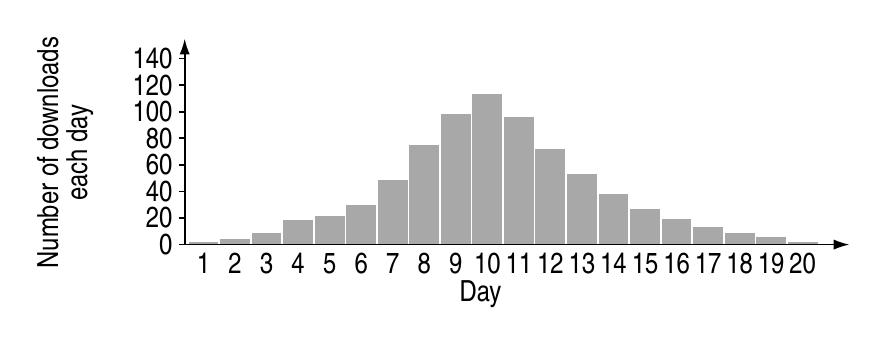
\begin{tikzpicture}[x=0.0127cm,y=0.0127cm,font=\fontsize{10.5}{12.6}\fontfamily{phv}\fontseries{mc}\selectfont]
  % bar tops and layout measured from the crop pixels (origin = foot of y-axis); same frame for options A-C
  %% bar heights (downloads, approx): 2, 5, 9, 19, 22, 30, 49, 75, 99, 114, 96, 72, 53, 38, 27, 20, 14, 9, 6, 2
  \fill[black!34, draw=white, line width=0.6pt] (3.0,0) rectangle (34.5,3);
  \fill[black!34, draw=white, line width=0.6pt] (34.5,0) rectangle (66.1,6);
  \fill[black!34, draw=white, line width=0.6pt] (66.1,0) rectangle (97.6,12);
  \fill[black!34, draw=white, line width=0.6pt] (97.7,0) rectangle (129.2,25);
  \fill[black!34, draw=white, line width=0.6pt] (129.2,0) rectangle (160.8,29);
  \fill[black!34, draw=white, line width=0.6pt] (160.8,0) rectangle (192.3,40);
  \fill[black!34, draw=white, line width=0.6pt] (192.3,0) rectangle (223.9,65);
  \fill[black!34, draw=white, line width=0.6pt] (223.8,0) rectangle (255.4,100);
  \fill[black!34, draw=white, line width=0.6pt] (255.4,0) rectangle (286.9,131);
  \fill[black!34, draw=white, line width=0.6pt] (286.9,0) rectangle (318.5,151);
  \fill[black!34, draw=white, line width=0.6pt] (318.5,0) rectangle (350.1,128);
  \fill[black!34, draw=white, line width=0.6pt] (350.1,0) rectangle (381.6,96);
  \fill[black!34, draw=white, line width=0.6pt] (381.6,0) rectangle (413.2,71);
  \fill[black!34, draw=white, line width=0.6pt] (413.2,0) rectangle (444.7,51);
  \fill[black!34, draw=white, line width=0.6pt] (444.7,0) rectangle (476.2,36);
  \fill[black!34, draw=white, line width=0.6pt] (476.2,0) rectangle (507.8,26);
  \fill[black!34, draw=white, line width=0.6pt] (507.8,0) rectangle (539.4,18);
  \fill[black!34, draw=white, line width=0.6pt] (539.4,0) rectangle (570.9,12);
  \fill[black!34, draw=white, line width=0.6pt] (570.9,0) rectangle (602.4,8);
  \fill[black!34, draw=white, line width=0.6pt] (602.5,0) rectangle (634.0,3);
  \draw[->] (-4,0) -- (665,0);
  \draw[->] (0,0) -- (0,206);
  \draw (-6,0.0) -- (0,0.0); \node[anchor=east, inner sep=2pt] at (-6,0.0) {0};
  \draw (-6,26.6) -- (0,26.6); \node[anchor=east, inner sep=2pt] at (-6,26.6) {20};
  \draw (-6,53.1) -- (0,53.1); \node[anchor=east, inner sep=2pt] at (-6,53.1) {40};
  \draw (-6,79.7) -- (0,79.7); \node[anchor=east, inner sep=2pt] at (-6,79.7) {60};
  \draw (-6,106.3) -- (0,106.3); \node[anchor=east, inner sep=2pt] at (-6,106.3) {80};
  \draw (-6,132.9) -- (0,132.9); \node[anchor=east, inner sep=2pt] at (-6,132.9) {100};
  \draw (-6,159.4) -- (0,159.4); \node[anchor=east, inner sep=2pt] at (-6,159.4) {120};
  \draw (-6,186.0) -- (0,186.0); \node[anchor=east, inner sep=2pt] at (-6,186.0) {140};
  \node at (18.8,-19) {1};
  \node at (50.3,-19) {2};
  \node at (81.9,-19) {3};
  \node at (113.4,-19) {4};
  \node at (145.0,-19) {5};
  \node at (176.5,-19) {6};
  \node at (208.1,-19) {7};
  \node at (239.6,-19) {8};
  \node at (271.2,-19) {9};
  \node at (302.7,-19) {10};
  \node at (334.3,-19) {11};
  \node at (365.8,-19) {12};
  \node at (397.4,-19) {13};
  \node at (428.9,-19) {14};
  \node at (460.5,-19) {15};
  \node at (492.0,-19) {16};
  \node at (523.6,-19) {17};
  \node at (555.1,-19) {18};
  \node at (586.7,-19) {19};
  \node at (618.2,-19) {20};
  \node at (296,-50) {Day};
  \node[rotate=90] at (-137,92) {Number of downloads};
  \node[rotate=90] at (-105,92) {each day};
\end{tikzpicture}
\end{document}
